%%%%%%%%%%%%%%%%%%%%%%%%%%%%%%%%%%%%%%%
% 3.1: proximal operator
% definitions, basics and algorithm
%%%%%%%%%%%%%%%%%%%%%%%%%%%%%%%%%%%%%%%

\subsection[Proximal operator]{Compute the proximal operator}

In many cases, to improve the computation cost of a function $f$, we consider the proximal mapping. Fast algorithm already exist to compute these objects such as FISTA \cite{beck2009fast}, the proximal gradient method \cite{ryu2017proximal}, \dots

% proximal operator
\begin{definition}[Moreau's proximal mapping]\label{def:prox}
Let $f$ be a real function, its proximal operator (or Moreau's proximal operator) $\prox_f$ is defined as follows:
\[\forall x\in\EE,\ \prox_f(x) =\arg\min_{u\in \EE}\left\{f(u) + \frac{1}{2}\|u-x\|^2_2\right\}\enspace.\] 
\end{definition}

This can be either a set of multiple elements, an empty set or a singleton. In our case, the following lemma and theorem assure that $\abs{\prox_{\mathcal{S}(x)}} = 1$. The proof is available in \cite{beck}.

% S_k is closed => needed for the singleton of prox
\begin{lemma}
The sparse envelope $\mathcal{S}_k$ is closed \emph{ie} for all $y \in \RR,\ \left\{x\in \mathcal{D}_f\, |\, f(x)\leq y\right\}$ is closed.
\end{lemma}
\begin{theorem}\label{thm:unicityprox}
For a proper closed convex function $f$, $\abs{\prox_f(x)} = 1$ for all $x\in\EE$.
\end{theorem}

When solving an inverse problem, as we saw with the ridge penalty or \enet, there is an hyperparameter multiplying the penalty factor. Let's note it $\lambda_s>0$ for the sparse envelope. Then theorem \ref{thm:unicityprox} still holds and there is an almost explicit formulation for the value of $\prox_{\lambda\mathcal{S}_k}$.

% form for the \lambda prox_k(x) with u_i 
\begin{proposition}\label{prop:wlambdaS}
From $u=\min\limits_{u\in D_k}\sum_{i=1}^n \phi(x_i,\lambda + u_i)$ with $\lambda > 0$, we can compute $w=\prox_{\lambda\mathcal{S}_k}(x)$ defined as:
\begin{equation}\label{eq:proxui}
    \forall\ i=1,\dots,n\ w_i=\frac{x_iu_i}{\lambda + u_i}\enspace.
\end{equation}
\end{proposition}
\begin{proof}
Using definition \ref{def:prox} followed by proposition \ref{prop:Sfromphi}, \[\begin{aligned}
w&=\arg\min_{z\in\RR^n}\left\{\lambda\mathcal{S}_k(z) + \frac{1}{2}\|z-x\|^2_2\right\} = \arg\min_{z\in\RR^n}\left\{\frac{\lambda}{2}\min_{u\in D_k}\sum_{i=1}^n\phi(z_i, u_i) + \frac{1}{2}\|z-x\|^2_2\right\}\\
&=\arg\min_{z\in\RR^n}\min_{u\in D_k}\underbrace{\left\{\frac{\lambda}{2}\sum_{i=1}^n\phi(z_i, u_i) + \frac{1}{2}\|z-x\|^2_2\right\}}_{\varphi}\enspace.
\end{aligned}\]
From there, we need to solve for $z$ the inner minimization. We note $\hat z$ the value at the optimum. Suppose that $u_i>0$ (otherwise $u_i=0=\hat z_i$), then from the first order condition for all $i_0=1,\dots,n$:
\[\begin{aligned}
\frac{\partial\varphi}{\partial z_{i_0}}(x, \hat z, u)= 0 &\Longleftrightarrow \frac{\lambda}{2}\frac{2\hat z_{i_0}}{u_{i_0}} + \frac{2}{2}(\hat z_{i_0} - u_{i_0})\\
& \Longleftrightarrow \hat z_{i_0} = \frac{u_{i_0}z_{i_0}}{\lambda + u_{i_0}}\enspace.
\end{aligned}\]
And plugging-in this result, it is easy to show that $\varphi(x,\hat z, u) = \frac{\lambda}{2}\sum_{i=1}^n \phi(x_i, \lambda + u_i)$.
\end{proof}

% Final theorem to get to the algorithm
If we try to compute the proximal operator with the formula from proposition \ref{prop:wlambdaS}, finding the vector $u$ directly is quite hard. We can simplify the search solving a one-dimensional problem as the following theorem states.

\begin{theorem}\label{thm:proxval}
For $x\in\RR^n$ and $\lambda>0$:
\begin{itemize}
    \item if $\|x\|_0\leq k$ then $w=\prox_{\lambda\mathcal{S}_k}(x)=\frac{1}{\lambda + 1}x$,
    \item if $\|x\|_0> k$ then $w_i=(\prox_{\lambda\mathcal{S}_k}(x))_i=\frac{x_iu_i}{\lambda + u_i}$.
\end{itemize}
To find the value of $u_i$, we define $h(\eta)=\sum_{i=1}^n \mathbf{u_i}(\eta) - k$, where the function $\mathbf{u_i}:\eta\mapsto\mathbf{u_i}(\eta)$ is:
\[\mathbf{u_i}(\eta)=\begin{cases}
0 & \text{ if }\eta \leq \frac{\lambda}{\abs{x_i}}\enspace,\\
\abs{x_i}\eta & \text{ if }\frac{\lambda}{\abs{x_i}}< \eta < \frac{\lambda  + 1}{\abs{x_i}}\enspace,\\
1 & \text{ if } \eta\geq \frac{\lambda+1}{\abs{x_i}}\enspace,
\end{cases} i=1,\dots,n\enspace.
\]
Then $u_i=\mathbf{u_i}(\tilde\eta)$, with $\tilde\eta$ defined such that $h(\tilde\eta)=0$.
\end{theorem}

%%% Introduce bisector method
So the issue is now to find the root of the function $h$. A first way to do so can be using the bisector algorithm. Indeed, we only need to find an interval to start off that contains the root because $h$ is continuous. And we can see that:
\[\begin{aligned}
&h\left(\frac{\lambda}{\|x\|_\infty}\right)=\sum_{i=1}^n \mathbf{u_i}\left(\frac{\lambda}{\|x\|_\infty}\right)-k = \sum_{i=1}^n 0 -k = -k < 0,\\
&h\left(\frac{\lambda+1}{\abs{x_{\langle \|x\|_0\rangle}}}\right) = \sum_{i=1}^n \mathbf{u_i}\left(\frac{\lambda+1}{\abs{x_{\langle \|x\|_0\rangle}}}\right) - k = \sum_{i:x_i\neq 0}\underbrace{\mathbf{u_i}\left(\frac{\lambda+1}{\abs{x_{\langle \|x\|_0\rangle}}}\right)}_{=1} = \|x\|_0-k \geq 0\enspace.
\end{aligned}\]

So we can simply apply the bisector method on the interval $\left[\frac{\lambda}{\|x\|_\infty}, \frac{\lambda + 1}{\abs{x_{\langle \|x\|_0\rangle}}}\right]$ to find $\tilde\eta$. However, we can also use the characteristics of the function $h$ to find such value, $h$ being the sum of piecewise linear functions with two breakpoints. That fact is exploited by the \textit{Random search} algorithm presented hereafter.

%%%%%%%%%%%%%%%%%%%%%%%%%%%%%%%%%%
% Algorithm to compute SE
%%%%%%%%%%%%%%%%%%%%%%%%%%%%%%%%%%

\subsection[Algorithm]{Algorithms for the sparse envelope}
To find the root of a function defined as the sum of piecewise linear functions with a single breakpoint, we can use the \textit{Random Search} algorithm. We note the function $F$, and assume it is monotonous, has a root and defined as \[F(x)=\sum_{j=1}^n F_j(x) - k\enspace,\] with $F_j(x)=\alpha^1_jx + \beta^1_j$ if $x\leq \gamma_j$ and $\alpha_j^2x+\beta_j^2$ otherwise, $j$ continuous functions.

\begin{figure}[H]
    \center
    
    \begin{tikzpicture}[node distance=1.5cm,
        every node/.style={fill=white, font=\sffamily}, align=center]
      % Specification of nodes (position, etc.)
      \node (start)[ activityStarts]{Input: $\alpha^2,\alpha^2, \beta^1 \beta^2\in \RR^n, \delta\in\RR$\\ $F=\sum_{i=1}^nF_j - \delta$};
      \node (beginning)[process, below of=start]{
      Init: $\Omega = \{1,\dots,n\}$\\ $\tilde\alpha=0$, $\tilde\beta=0$};
      \node (while)[process, below of=beginning]{
      While $\Omega\neq\emptyset$:\\
      Pick randomly $p\in\Omega$\\
      $F(\gamma_p)\leftarrow \tilde\alpha\gamma_p + \tilde\beta + \sum_{j\in\Omega}F_j(\gamma_p)$};
      \node(pos)[process, below of=while, yshift=-1.5cm, xshift=-4cm]{
      If $F(\gamma_p)>0$:\\
      $A\leftarrow \{j\in\Omega\,|\, \gamma_j<\gamma_p\}$\\
      $\tilde\alpha\leftarrow \tilde\alpha + \sum_{j\in\Omega\setminus A}\alpha_j^1$\\
      $\tilde\beta \leftarrow \tilde\beta + \sum_{j\in \Omega\setminus A}\beta_j^1$\\
      $\Omega\leftarrow A$};
      \node(neg)[process, below of=while, yshift=-1.5cm, xshift=+4cm]{
      If $F(\gamma_p)<0$:\\
      $A\leftarrow \{j\in\Omega\,|\, \gamma_j>\gamma_p\}$\\
      $\tilde\alpha\leftarrow \tilde\alpha + \sum_{j\in\Omega\setminus A}\alpha_j^2$\\
      $\tilde\beta \leftarrow \tilde\beta + \sum_{j\in \Omega\setminus A}\beta_j^2$\\
      $\Omega\leftarrow A$};
      \node(end0)[startstop, below of=while, yshift=-1.5cm]{If $F(\gamma_p)=0$:\\ \textbf{Return}: $\eta^*=\gamma_p$};
      \node(endwhile)[startstop, below of=end0, yshift=-.7cm]{
      \textbf{Return:} $\eta^*=-\tilde\beta / \tilde\alpha$};
      
      % draw the lined
      \draw[->] (start)   --  (beginning);
      \draw[->] (beginning)   --  (while);
      \draw[->] (while) -- (pos);
      \draw[->] (while) -- (neg);
      \draw[->, dotted, line width=2pt] (pos) --++ (0,3) --++ (while);
      \draw[->, dotted, line width=2pt] (neg) --++ (0,3) --++ (while);
      \draw[->] (while) -- (end0);
      \draw[->] (while.north west) --++(3,0) -- node[right]{If $\Omega=\emptyset$} ++(6,0) |- (endwhile);
    
      \end{tikzpicture}
      
      \label{fig:algorand}
      \caption{Diagram for the random search algorithm procedure.}
      
    \end{figure}

This algorithm exploits the fact that $F$ is monotonous and its continuity. We eject cases that are not possible \textit{ie} if for a value $\gamma_{i_0}$ the function is strictly positive, then all values over $\gamma_{i_0}$ will lead to a positive result. Then the root must be before $\gamma_{i_0}$. If a value in $\gamma$ leads to a null result, then it is the root. Otherwise, we apply the algorithm until no one is left and find ourselves finding the root of an affine function.

\begin{remark}
Note that this algorithm exploits the fact that the problem was reduced from finding a vector of dimension $n$ to finding the root of a function in one dimension. Besides, it is efficient with sparse vectors because of the choice of the $F_j$ functions in the sum. In the worse case, we find ourselves with a complexity of $\mathcal{O}(n)$ that does not depend on the size of an initial interval like the bisection method.
\end{remark}

The problem is, the function $h$ defined in theorem \ref{thm:proxval} is the sum of piecewise linear functions with two breakpoints. So to use the \textit{Random search}, we need to decompose $h$ as the following lemma states.

\begin{lemma}
We can decompose $h$ into the sum of at most $2n$ piecewise linear functions with a single breakpoint:
\[h(\eta)=\frac{1}{2}\sum_{i:x_i\neq 0}\abs{\eta\abs{x_i}-\lambda} +\frac{1}{2}\sum_{i:x_i\neq 0}\left(1-\abs{\eta \abs{x_i} - \lambda - 1}\right) - k\enspace.\]
\end{lemma}

% Example of the soft threshold
To understand this decomposition on a simpler function, we can look at $G\,:\,\RR\rightarrow\RR$:

\[G(x)=\begin{cases} 0& \text{ if }x\leq 0,\\
                    x & \text{ if }x\in]0,1[\\
                    1 & \text{ if }x\geq 1\end{cases}\enspace.\]
As represented in Figure \ref{fig:decomposition}, $G$ can be written as $\frac{1}{2}G_1 + \frac{1}{2}G_2$ taking
\[G_1(x)=\abs{x} \quad\text{and}\quad G_2(x)=1-\abs{x-1}\enspace.\]
% figure for decomposition into sum of single-breakpoints
\begin{figure}[H]
    \centering
    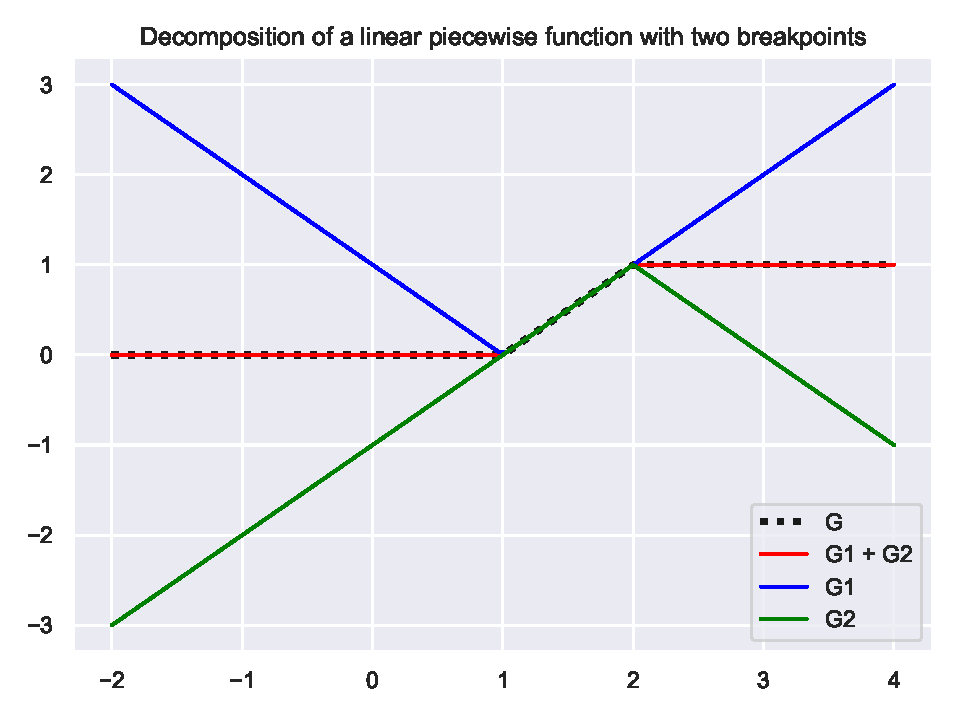
\includegraphics[height=7cm, trim={0cm 0Cm 0cm 1cm}, clip]{decomposition.pdf}
    \caption{Decomposition of a piecewise linear signal with two breakpoints into the sum of two piecewise learn signals with a single breakpoint each.}
    \label{fig:decomposition}
\end{figure}

And more generally (as we need to split $h$) for a continuous function $G$ defined such that $G(x)= mx + n$ if $x\in ]\alpha, \beta[$, $0$ if $x\leq \alpha$ and $1$ if $x\geq\beta$, we have:
\[G_1(x)=m\abs{x-\alpha} \quad\text{and}\quad G_2(x)=1-m\abs{x-\beta}\enspace.\]

% Like with function evaluation
\begin{remark}
The algorithm presented can not only be used to find the root of the function $h$, but also to solve equation \eqref{eq:applyalgofunc} that finds the value of $\mathcal{S}_k(x)$. Notice that in this case, there is no need for a decomposition as the functions only have a single breakpoint. We can just apply the random search with $\alpha_j^1=\abs{x_j}$, $\alpha_j^2=0$, $\beta_j^1=0$ and $\beta_j^2=1$. Then $\gamma_j=\abs{x_j}^{-1}$ and $\delta=k$. As the function in the sum was $\min\{\abs{x_i}\eta,1\}$, the functions $F_j$ are defined as:
\[F_j(\eta)=\begin{cases}\abs{x_i}\eta,\text{ if }\frac{1}{\abs{x_i}}\geq \eta, \\ 1 \text{ otherwise}\end{cases}\enspace.\]
Note that the sparsity of the vector can be taken into account by only considering the subset $\{i\,|\, x_i\neq 0\}\subseteq \{1,\dots,n\}.$
\end{remark}

%%%%%%%%%%%%%%%%%%%%%%%%%%%%%%%%%%
% Numerical results part : 
%%%%%%%%%%%%%%%%%%%%%%%%%%%%%%%%%%
\subsection{Numerical application}

Let's finally compare our regularized problem with the \enet
regularization in an highly correlated situation (the same represented in Figure \ref{fig:lasso_enet}).
We simulate a signal with only $3$'s for the first fifteen components and zeros for the $25$ left. The observed signal is 
\[ b = Ax + \varepsilon\enspace,\]
where $\varepsilon\sim\mathcal{N}(0,\sigma^2)$ is a Gaussian noise.
The matrix $A$ is constructed from the algorithm that follows so that we can recreate the grouping effect:
\begin{itemize}
\setlength{\arraycolsep}{1pt} % resize matrices
    \item generate three random vectors $z_1,\ z_2$ and $z_3\in\RR^n$,
    \item from $z_i$, compute $Z_i=\begin{bmatrix} z_i, & z_i, & z_i, & z_i, & z_i\end{bmatrix}\in\RR^{n\times 5}$,
    \item generate $B,\ C,\ D\in\RR^{n\times 5}$ and $E\in\RR^{n\times 25}$,
    \item $A=\begin{bmatrix}Z_1 + 0.01 W_1, & Z_2 + 0.01 W_2, & Z_3 + 0.01 W_3, & E \end{bmatrix}$.
\end{itemize}
Doing so, we find ourselves with a matrix $A$ which has groups of vectors very similar (the first five vectors are almost equal, as are the next five and the next five after). With the \lasso we saw in Figure \ref{fig:lasso_enet} that the algorithm decides to select one in each group. The \enet is made to counterbalance that effect, so is the sparse envelope.

%%%%%%%%%%% End the data preparation %%%%%%%%%%%%%
%%%%%%%%%%% Begin numerical analysis %%%%%%%%%%%%%

The sparse-envelope problem is written as:
\[\min_{x\in \RR^n} \|Ax-b\|^2_2 + \lambda\mathcal{S}_k(x)\enspace,\]
where $\lambda$ must be chosen through a train/test procedure and we take $k=15$ because we know its real value here. Otherwise we would have to search it as well.

\medskip

As the Figure \ref{fig:enet_sp} shows, the proximal envelope is closer to the original signal than the \enet in this case.
We can now compare if this is also the case for some values of $n\in\NN^*$ and quantify the gain of using this method instead of the \enet.


% Figure enet and prox signal together
\begin{center}
    \begin{figure}[H]
        \centering
        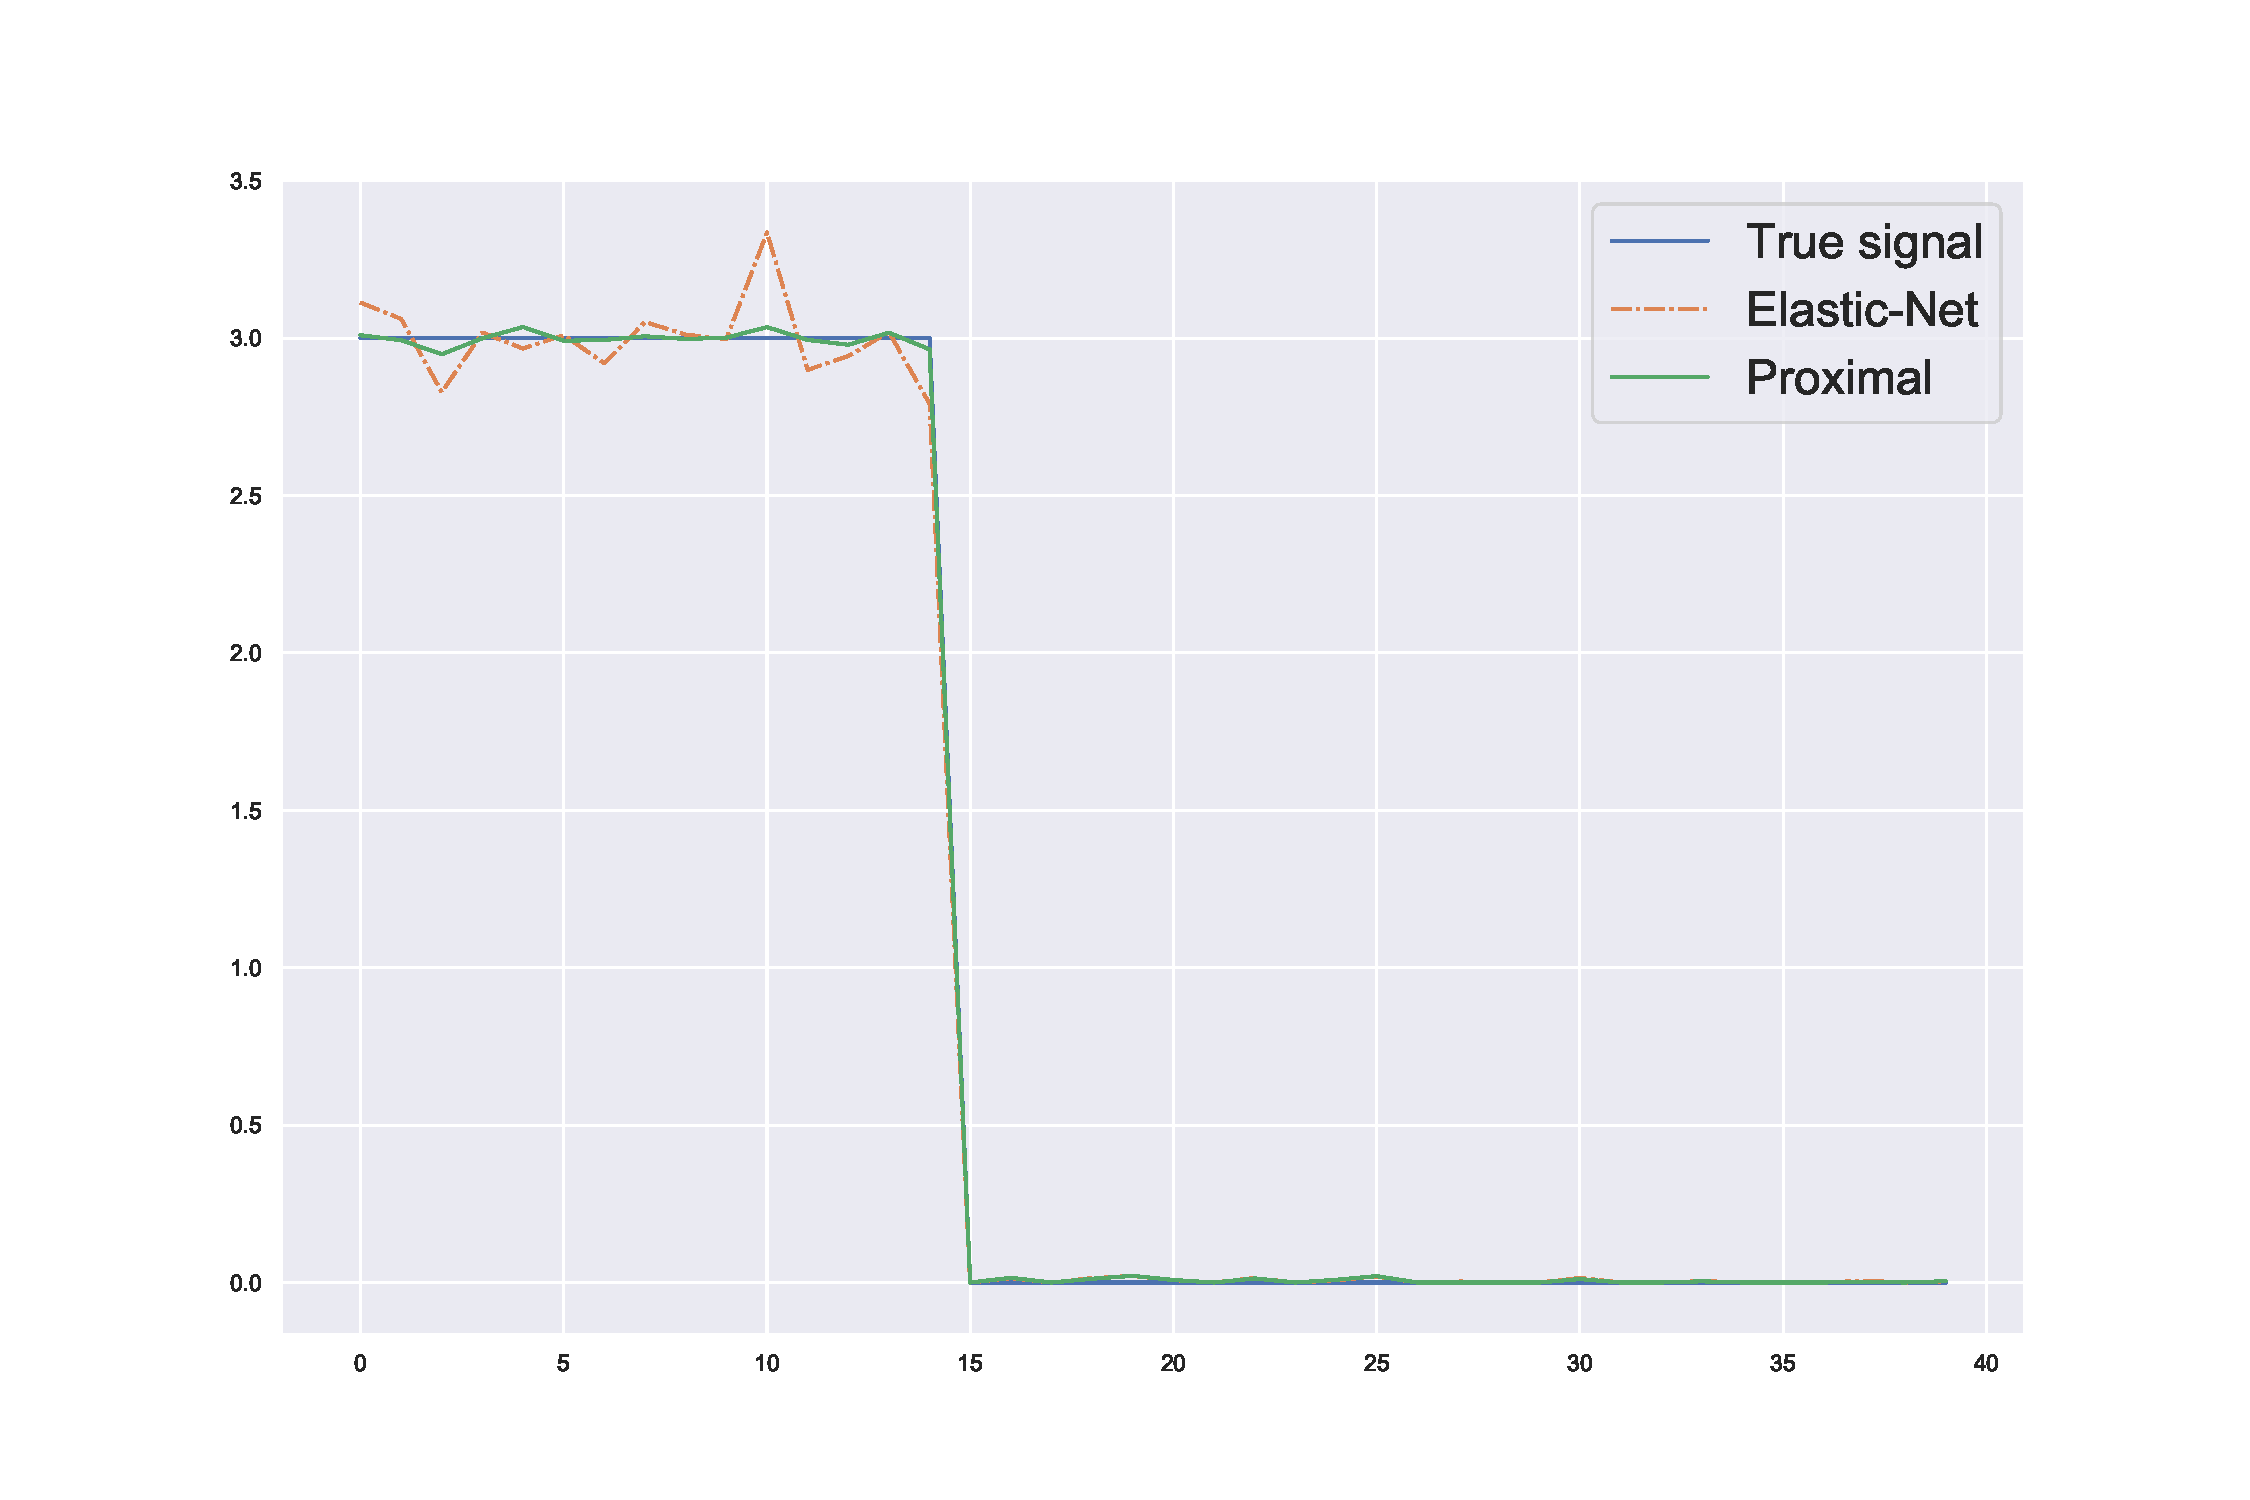
\includegraphics[width=.9\linewidth]{enet_proxi.pdf}
        \caption{Comparison of the Elastic-net and sparse regularization in a highly correlated situation with $n=50$ and $\sigma=0.1$.}
        \label{fig:enet_sp}
    \end{figure}
\end{center}

\begin{remark}
To compute the sparse envelope method, we used the FISTA algorithm using the $2-$norm of the matrix $A$ for the Lipschitz constant.
\end{remark}

\paragraph*{}
%% Table of the results for the diminution of the residuals
To do so, we call $x_{enet}$ the solution returned by the \enet method and $x_{prox}$ the one returned by the method we described. The residuals are respectively $\|x-x_{enet}\|_2$ and $\|x-x_{prox}\|_2$ for both methods. Finally, we want to look at the improvement made by the latter against the former. So the percentage of improvement of the residuals is given by:
\[\mathrm{IM}(x_{prox}\,||\,x_{enet})=\left(\frac{\|x-x_{prox}\|_2}{\|x-x_{enet}\|_2} - 1 \right) \times 100\enspace.\]

To see different cases, we tried $n\in\{40, 80\}$ and $\sigma\in\{0.1,1,2\}$.
We generated new data for $A$ (and therefore $b$) $J=50$ times for each experiment, the improvements percentages showed are defined as
\[\bar{\mathrm{IM}}_{n}(J) = \frac{1}{J}\sum_{j=1}^J \mathrm{IM}(x_{prox}^{(j)}\,||\, x_{enet}^{(j)})\enspace.\]

\begin{remark}
A negative improvement in this case means that the error was reduced from the \enet to the sparse envelope method. If the sparse envelope method were perfect and resulted in $x=x_{prox}$, then $\mathrm{IM}(x_{prox}\,||x_{enet})=-100\%$. \end{remark}

In addition to the mean of the improvements, we provide the standard deviation needed for the confidence interval (each simulation is indeed independent of the previous ones and we generate the data with normal distributions of fixed parameters for a chosen $\sigma$).

% results table: SE way better in this case
\begin{table}[H]
    \centering
    \begin{tabular}{cccc}
    $n$ & $\sigma$ & $\bar{\mathrm{IM}}_n(50)$ & $\hat\sigma\left(\mathrm{IM}_n(50)\right)$\\
    \hline
    $40$     &  $0.1$ & $-98.55\%$ & $0.510$ \\
             &  $1.0$ & $-98.29\%$ & $0.543$\\
             &  $2.0$ & $-97.75\%$ & $0.768$\\  \hline
    $80$     &  $0.1$ & $-99.09\%$ & $0.308$\\
             &  $1.0$ & $-99.15\%$ & $0.361$\\
             &  $2.0$ & $-98.79\%$ & $0.580$\\
    \end{tabular}
    \caption{Average improvement obtained comparing for the residuals of the inverse problem using the \enet method against the sparse envelope.}
    \label{tab:endresults}
\end{table}

From Table \ref{tab:endresults} and Figure \ref{fig:enet_sp}, we can conclude that in situations involving a grouping effect, the sparse envelope has a better accuracy than the \enet. However, the bigger the noise, the closer the two method get (especially on the part of the signal where the true signal equals zero). 
